\chapter{Supercomputers}

Modern scientific discovery increasingly relies on high-performance computing infrastructure capable of handling massive computational workloads. Supercomputers represent the pinnacle of this infrastructure, combining thousands of processors, accelerators, and specialized networking hardware to tackle problems that would be intractable on conventional systems. These range from climate modeling and molecular dynamics simulations to machine learning training and quantum mechanics calculations.
We will focus on Leonardo, one of Europe's flagship supercomputing systems. We'll examine its modular design, computing capabilities, and the practical aspects of accessing and utilizing it.

\section{Leonardo Supercomputer}

Leonardo is a pre-exascale supercomputer hosted at CINECA in Bologna, Italy, and represents one of the cornerstones of the European High Performance Computing Joint Undertaking (EuroHPC JU). Leonardo was designed to support both traditional HPC workloads and emerging AI applications.

The system exemplifies the trend toward heterogeneous computing in modern HPC, integrating both CPU-centric compute nodes and GPU-accelerated nodes optimized for highly parallel workloads.

\subsection{System Architecture and Modules}

Leonardo adopts a modular architecture consisting of several distinct partitions, each tailored to specific classes of workloads. The two primary modules are the \textbf{Booster module} and the \textbf{Data-Centric (DHPC) module}, supplemented by additional service and hybrid partitions.

\subsubsection{Booster Module}

The Booster module constitutes the heart of Leonardo's computational power and is optimized for massively parallel, compute-intensive workloads. This partition is composed of GPU-accelerated nodes, each equipped with:

\begin{itemize}
    \item \textbf{CPUs}: 1 Intel Xeon Platinum 8358 processor (32 cores, 2.6 GHz base frequency)
    \item \textbf{GPUs}: 4 NVIDIA A100 GPUs (64 GB HBM2 memory each), providing substantial computational throughput for floating-point operations and tensor computations
    \item \textbf{System Memory}: 512 GB DDR4 RAM per node
    \item \textbf{Node-to-GPU Interconnect}: GPUs connected via NVIDIA NVLink for high-bandwidth, low-latency communication within each node
\end{itemize}

The Booster module comprises approximately 3,500 such nodes, yielding roughly 14,000 NVIDIA A100 GPUs in total. This configuration is particularly well-suited for applications in machine learning, computational fluid dynamics, materials science, and other domains that benefit from the massive parallelism offered by modern GPUs. Each A100 GPU provides mixed-precision capabilities (FP64, FP32, FP16, and Tensor Core operations), enabling efficient execution of both traditional HPC simulations and AI training workloads.

\subsubsection{Data-Centric (DHPC) Module}

The Data-Centric module provides CPU-centric compute resources designed for workloads that require large memory capacity, complex branching logic, or I/O-intensive operations. Nodes in this partition feature:

\begin{itemize}
    \item \textbf{CPUs}: 2 Intel Xeon Platinum 8358 processors per node (64 cores total)
    \item \textbf{System Memory}: Typically 512 GB DDR4 RAM per node, with some high-memory configurations available
    \item \textbf{Local Storage}: NVMe SSDs for fast local data staging
\end{itemize}

This module comprises approximately 1,500 nodes and is intended for traditional HPC applications such as computational chemistry codes, finite element analysis, and large-scale data analytics tasks that do not map efficiently onto GPU architectures.

\subsubsection{Inter-Node Network Topology}

\vspace{-0.5em}

\begin{minipage}{0.67\textwidth}
Leonardo employs a \textbf{Dragonfly+} network topology based on NVIDIA Mellanox InfiniBand HDR (High Data Rate) technology and NVIDIA Quantum QM8700 switches. This topology is designed to provide high bandwidth and low latency while maintaining scalability and resilience.

\medskip

In the Dragonfly+ topology, compute nodes are organized into \textbf{groups} (or cells), with dense all-to-all connectivity within each group. Inter-group connections are carefully engineered to minimize the maximum number of hops between any two nodes while balancing cost and performance. Each node is connected via InfiniBand HDR links operating at 200 Gb/s, ensuring that communication-intensive parallel applications can scale efficiently across thousands of nodes.
\end{minipage}%
\hfill
\begin{minipage}{0.3\textwidth}
    \vspace{-2.5em}
\begin{figure}[H]
    \centering
    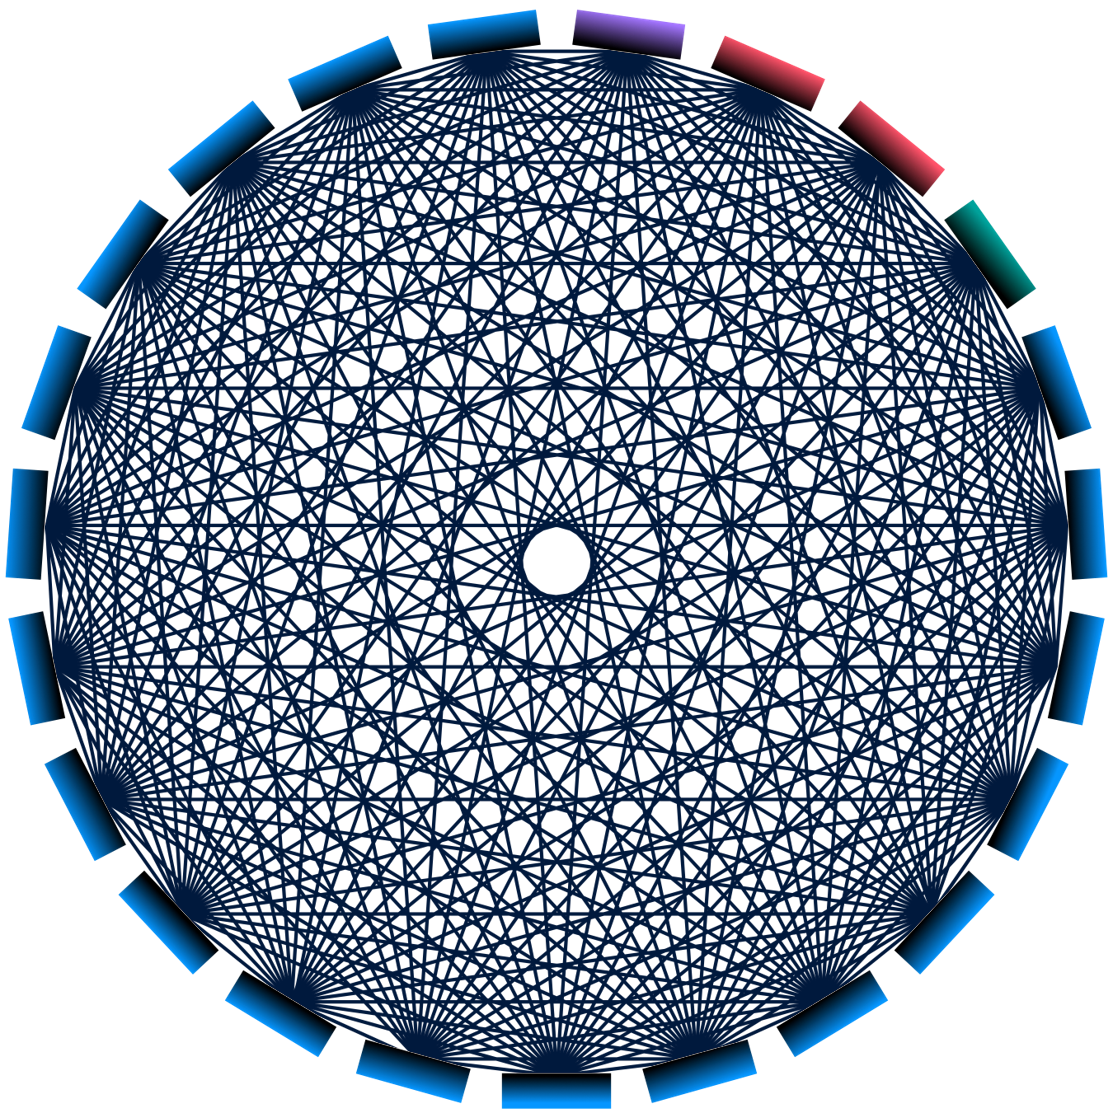
\includegraphics[width=\textwidth]{assets/leo-topology.png}
    \caption{Dragonfly+ Topology. Booster Module nodes (blue), I/O cell (purple), Data-centric cells (red), and Hybrid cell (green).}
    \label{fig:dragonfly-topology}
\end{figure}
\end{minipage}

\subsection{Storage System}

Leonardo's storage infrastructure is organized into a two-tier hierarchy:

\begin{itemize}
    \item \textbf{Fast Tier (NVMe-based)}: 5.4 PB of capacity with an aggregate bandwidth of 1.4 TB/s. This tier uses high-speed NVMe SSDs and is intended for I/O-intensive workloads requiring rapid data access, such as checkpointing in large-scale simulations or intermediate data staging for machine learning training.
    
    \item \textbf{Capacity Tier (HDD-based)}: 106 PB of capacity with an aggregate bandwidth of 2.9 TB/s. This tier provides long-term storage for datasets, simulation outputs, and archival purposes. While slower than the fast tier, it offers significantly greater capacity at a lower cost per terabyte.
\end{itemize}

Both tiers are accessible via a parallel filesystem (typically GPFS/Spectrum Scale or Lustre) that provides a unified namespace and supports concurrent access from thousands of compute nodes.

\begin{observationblock}[Top500]
    The \textbf{Top500} list is the authoritative ranking of the world's fastest supercomputers, updated twice a year (June and November). Leonardo currently holds the rank of 9th fastest supercomputer globally. At its debut in November 2022, Leonardo achieved the impressive position of \textbf{4th fastest}, trailing only Frontier (USA), Fugaku (Japan), and LUMI (Finland).

\end{observationblock}

\subsection{Accessing Leonardo}

Access to Leonardo is managed through a project-based allocation system. For users affiliated with Italian universities and research institutions, CINECA offers several account classes tailored to different project sizes and durations:

\begin{tipsblock}[Apply for resources]
    If you belong to an Italian university, you can apply for resources in the following classes:
    \begin{itemize}
        \item \textbf{Class B}: Large-scale projects, typically requesting millions of core-hours. Duration: 12 months. Calls for proposals are issued twice per year.
        \item \textbf{Class C}: Small to medium-sized projects. Duration: 9 months. Continuous submission process, with up to 10 calls per year.
        \item \textbf{Class D}: Storage allocations related to HPC simulations, useful for projects requiring substantial long-term data retention. Duration: 36 months.
        \item \textbf{Test Account}: Small allocations for testing, debugging, and scaling studies. Duration: 3 months. Ideal for validating code performance before requesting larger allocations.
    \end{itemize}
\end{tipsblock}

    \medskip

Upon logging in to Leonardo, users are greeted by the \textbf{Message of the Day} (MOTD), an informational banner designed to keep users up-to-date with the system's status and important announcements. The MOTD typically includes:
\begin{itemize}
    \item A brief description of the cluster architecture or key features
    \item Real-time system status updates (e.g., queues, ongoing issues, resource availability)
    \item ``In evidence'' messages highlighting noteworthy news or actionable items
    \item Important notifications, such as planned downtime, upcoming maintenance, or urgent advisories
\end{itemize}

\section{Working on Leonardo}

\subsection{Filesystem Organization}

Upon logging into Leonardo, users find themselves in a hierarchical filesystem with several designated directories, each serving a specific purpose:

\begin{itemize}
    \item \textbf{HOME} (\texttt{\$HOME}): A personal home directory; it is backed up and is intended for configuration files, scripts, and small datasets. Quota-limited, typically to tens of gigabytes.
    
    \item \textbf{WORK} (\texttt{\$WORK}): A larger, project-specific workspace for active development, source code, and intermediate build artifacts. Not typically backed up, but persistent across sessions.
    
    \item \textbf{SCRATCH} (\texttt{\$SCRATCH}): A high-performance scratch space for temporary files generated during job execution. This area offers the best I/O performance and is intended for files needed only during the runtime of a job. Files in scratch are subject to automatic purging policies (e.g., files not accessed for 40 days may be deleted), so do not use this for long-term storage.
    
    \item \textbf{DATA} (\texttt{\$DATA}): Intended for long-term storage of large datasets and simulation outputs. This directory is often mapped to the capacity storage tier and may have different quota and performance characteristics than \texttt{\$SCRATCH}.
    
    \item \textbf{PUBLIC}: A shared directory where project members can exchange data and scripts. Useful for collaboration within a project team.
\end{itemize}

Active simulation I/O should target \texttt{\$SCRATCH} for speed, while final results should be moved to \texttt{\$DATA} or \texttt{\$WORK} for safekeeping.

\subsection{Software and Module Environment}

Leonardo's software stack is managed via the \textbf{Environment Modules} system, with packages built and deployed using the \textbf{Spack} package manager. This approach allows for coexistence of multiple versions and configurations of libraries and compilers, enabling reproducibility and flexibility.

Upon login, a default environment is loaded, but users typically need to load additional modules to access specific compilers, MPI implementations, or scientific libraries. 

The module system provides commands to query, load, and manage the software environment:

\begin{itemize}
    \item \texttt{module avail} or \texttt{module av}: List all available modules.
    \item \texttt{module list}: Show currently loaded modules and profiles.
    \item \texttt{module load <name>}: Load a specific module into the environment.
    \item \texttt{module unload <name>}: Unload a module.
    \item \texttt{module purge}: Remove all loaded modules (useful for starting with a clean environment).
    \item \texttt{module show <name>}: Display information about what a module does (env. variables, paths).
    \item \texttt{modmap -m <name>}: Search or map module names (CINECA-specific tool).
\end{itemize}

Different \textit{profiles} or module collections may be available depending on whether you are working on CPU-only or GPU-enabled nodes, or whether you are using a specific programming model (MPI, CUDA, OpenMP, OpenACC, etc.).

\subsubsection{Programming Environments}

Leonardo supports multiple compiler toolchains and programming environments:

\begin{itemize}
    \item \textbf{GNU Compiler Collection (GCC)}: Open-source compilers (\texttt{gcc}, \texttt{g++}, \texttt{gfortran}).
    \item \textbf{NVIDIA HPC SDK}: Provides \texttt{nvc}, \texttt{nvc++},  \texttt{nvcc}, \texttt{nvfortran} with OpenACC and CUDA support, essential for GPU programming on the Booster module.
    \item \textbf{Intel oneAPI}: Compilers (\texttt{icc}, \texttt{icpc}, \texttt{ifort}) optimized for Intel CPUs, along with Intel MPI.
\end{itemize}

To develop GPU-accelerated code, load the NVIDIA HPC SDK module (e.g. \texttt{module load nvhpc}) and ensure that the CUDA runtime libraries are accessible. For traditional MPI applications, load an MPI module compatible with the chosen compiler (e.g. \texttt{module load openmpi}).

\begin{warningblock}[Intel and NVIDIA Compilers]
    \textbf{Important:} Intel compilers do \emph{not} support CUDA or GPU offloading on NVIDIA GPUs. If your code targets NVIDIA GPUs using CUDA, OpenACC, or similar technologies, you must use the NVIDIA HPC SDK tools for compilation.
\end{warningblock}

\subsection{Job Submission with Slurm}

CINECA HPC clusters, such as Leonardo, are shared among many users. As such, responsible usage is essential to ensure fair access and optimal performance for everyone. The system is divided into two main types of nodes: login nodes and compute nodes.

When you log in, you access a \textbf{login node}, intended only for light tasks such as editing files, compiling code, or performing brief test runs. Running heavy computations or large parallel jobs directly on it is strictly prohibited. The login environment enforces a hard CPU time limit for any process, and jobs exceeding this limit may be killed without warning. Furthermore, GPUs are not available on login nodes, so you cannot test or run GPU code interactively in this environment.

All resource-intensive and production workloads must be submitted to the \textbf{compute nodes} through the \bfit{Slurm} job scheduler. Slurm manages how resources like CPU cores, GPUs, memory, and temporary storage are allocated to different users. Compute nodes support two main job submission styles: batch mode, in which you provide a job script for Slurm to execute, and interactive mode, where you request an interactive session on a compute node for active development or debugging.

While compute nodes themselves are shared across users, once Slurm assigns resources to a job, those resources are dedicated exclusively to that job for its duration. It is crucial to request only the resources you truly need and to release them promptly to maximize efficiency and minimize costs, since accounting is based on \textit{reserved} resources rather than those you actively use.

\subsubsection{Batch Job Submission}

A typical batch script for Slurm on Leonardo includes a shebang line, a series of \texttt{\#SBATCH} directives specifying resource requirements, environment setup commands (loading modules), and finally the execution command. Below is an example for a GPU job:

\begin{codeblock}[language=bash]
#!/bin/bash

# Slurm directives
#SBATCH --job-name=my_gpu_job           # Job name
#SBATCH --nodes=1                       # Number of nodes
#SBATCH --ntasks-per-node=1             # Number of MPI tasks per node
#SBATCH --cpus-per-task=8               # Number of CPU cores per task
#SBATCH --gres=gpu:4                    # Request 4 GPUs per node
#SBATCH --mem=494000                    # Memory in MB (approx 480 GB)
#SBATCH --time=00:30:00                 # Wall-clock time limit (hh:mm:ss)
#SBATCH --partition=boost_usr_prod      # Partition (queue) to submit to
#SBATCH --account=tra25_gputs           # Account/project code
#SBATCH --reservation=s_tra_gputs       # (Optional) reservation name
#SBATCH --output=job_\%j.out             # Standard output file (\%j = job ID)
#SBATCH --error=job_\%j.err              # Standard error file

# Load necessary modules
module purge
module load nvhpc cuda

# Run the executable
srun ./my_application
\end{codeblock}

Key directives:

\begin{itemize}
    \item \texttt{-{}-nodes} and \texttt{-{}-ntasks-per-node}: Define the number of nodes and MPI ranks per node.
    \item \texttt{-{}-cpus-per-task}: Useful for hybrid MPI+OpenMP jobs. Each MPI rank (task) will have access to this many CPU cores.
    \item \texttt{-{}-gres=gpu:N}: Request \texttt{N} GPUs per node. On Booster nodes, typically \texttt{gpu:4} since each node has 4 A100 GPUs.
    \item \texttt{-{}-time}: Maximum wall-clock time. Jobs exceeding this limit are terminated.
    \item \texttt{-{}-partition}: Specifies the queue or partition. Common partitions on Leonardo include \texttt{boost\_usr\_prod} (Booster nodes) and \texttt{dcgp\_usr\_prod} (DHPC nodes).
    \item \texttt{-{}-account}: Your project or account code, used for tracking resource usage and billing.
\end{itemize}

To submit the job, save the script (e.g., \texttt{job.sh}) and run:

\begin{codeblock}[language=bash]
sbatch job.sh
\end{codeblock}

Slurm will return a job ID, which you can use to track the job's status.

\subsubsection{Interactive Jobs}

For debugging, performance profiling, or exploratory work, you may request an interactive session on compute nodes. Use \texttt{salloc} or \texttt{srun} with the \texttt{-{}-pty} option:

\begin{codeblock}[language=bash]
salloc --nodes=1 --ntasks-per-node=1 --cpus-per-task=8 --gres=gpu:1 \
       --time=01:00:00 --partition=boost_usr_prod --account=<your_account>
\end{codeblock}

Once the allocation is granted, you will receive an interactive shell on a compute node, where you can run and test your code interactively. Remember to exit or cancel the allocation when done to avoid wasting resources.

\subsubsection{Monitoring and Managing Jobs}

Slurm provides several commands for job monitoring and control:

\begin{itemize}
    \item \texttt{squeue -u <username>} or \texttt{squeue --me}: Display the status of your jobs (pending, running, etc.).
    \item \texttt{scontrol show job <jobid>}: Show detailed information about a specific job, including resource allocation, start time, and node assignments.
    \item \texttt{scancel <jobid>}: Cancel a running or pending job.
    \item \texttt{sacct -j <jobid>}: Retrieve accounting information for completed jobs, useful for post-mortem analysis of resource usage.
\end{itemize}

Use these commands to track your jobs, troubleshoot issues, and ensure efficient use of allocated resources.

%%%%%%%%%%%%%%%%%%%%%%%%%%%%%%%%%%%%%%%%%%%%%%%%%%%%%%%%%%%%%%%%%%%%%%%%%%%%%%%

\section{Accelerated Computing with CUDA C/C++}

\subsection{Introduction}

\begin{itemize}
    \item \textbf{Bandwith}: ...
    \item \textbf{Latency}: ...
    \item \textbf{Throughput}: ...
\end{itemize}

\subsubsection{Data management}

The more the data is closer to the GPU, the better the performance. Fast memory is very close to the cpu, but it is limited in size (registers, cache, L1, L2, L3, DRAM, storage).

The core idea in computer is to virtualize the memory and load it on DRAM, and then in cache, only when needed. 

In multicore architectures, the L3 cache and the DRAM are shared between the cores. Therefore, different tasks may want to access the same data, and wait for the others to finish.

\begin{warningblock}{Architecture and programming models}
    Changing in the architecture level also requires changes in the programming models to be efficient.
\end{warningblock}

\subsection{GPU Architecture}

In a node we have a \textbf{Host device} (CPU) and a \textbf{GPU device}. The GPU is connected to the Host via a PCIe bus. It is needed to transfer the data (off-load) from the Host to the GPU and vice versa.

GPUs does not launch a single thread, but a group of 32 threads all at once.

GPUs have a simple control, they do easy computations, but highly parallelizable.
 
\subsubsection{NVIDIA Ampere Architecture}

Each node contains multiple GPC (Graphics Processing Clusters), made up of multiple SM (Streaming Multiprocessors).

\begin{figure}[H]
    \centering
    \includegraphics[width=0.8\textwidth]{assets/nvidia-ampere.png}
    \caption{NVIDIA Ampere Architecture}
    \label{fig:nvidia-ampere}
\end{figure}

\begin{minipage}{0.6\textwidth}
    \todo{NVIDIA Streaming Multiprocessor description}
\end{minipage}%
\hfill
\begin{minipage}{0.38\textwidth}
\begin{figure}[H]
    \centering
    \includegraphics[width=\textwidth]{assets/nvidia-sm.png}
    \caption{NVIDIA Streaming Multiprocessor}
    \label{fig:nvidia-sm}
\end{figure}
\end{minipage}

% CUDA launches warps of 32 threads, dividing them into smaller groups.

\newpage

\subsection{CUDA Programming Model}

\texttt{<<<>>>}: are used to quantify the number blocks and threads to launch the kernel.

We have dirrerent qualifiers for the functions:
\begin{itemize}
    \item \texttt{\_\_global\_\_}: It indicates that the function will run in the GPU, and can be invoked generally both from the host and the device.

\begin{codeblock}[language=C]
__global__ void GPUFunction() {
    printf("Hello from GPU!\n");
}

int main() {
    CPUFunction();
    GPUFunction<<<1, 1>>>();
    cudaDeviceSynchronize();
}
\end{codeblock}

    \item \texttt{\_\_device\_\_}: device function, executed on the device.
    \item \texttt{\_\_host\_\_}: host function, executed on the host.
    \item \texttt{\_\_host\_\_ \_\_device\_\_}: host and device function, compiled for both.
\end{itemize}

A cuda kernel is executed as a grid (array) of threads, each of them runs in the same kernel.

Each thread has a unique index \texttt{threadIdx.x}, which is used to access the data.

To compile a program we must use the NVIDIA \texttt{nvcc} compiler. It is able to identify the functions to be executed on the GPU and the ones to be executed on the host.

\begin{codeblock}[language=bash]
nvcc -arch=sm_80 -o <output-file> <cuda-code>.cu -run
\end{codeblock}

Where:
\begin{itemize}
    \item \texttt{-arch=sm\_80}: specifies the architecture of the GPU to compile for.
    \item \texttt{-run}: runs the program after compilation.
\end{itemize}

\subsubsection{SIMT vs SIMD}

In cuda programming, we use the SIMT (Single Instruction Multiple Thread) model.

\begin{figure}[H]
    \centering
    \includegraphics[width=0.45\textwidth]{assets/simt.png}
    \caption{SIMT vs SIMD}
    \label{fig:simt-simd}
\end{figure}

\begin{itemize}
    \item \textbf{SIMD}: “One instruction, one data chunk.”
    \begin{itemize}
        \item A single instruction operates on multiple data elements simultaneously
        \item Requires wide vector units in hardware (e.g., 4 or 8 lanes)
        \item A SIMD register (or a vector register) can hold many values (2 - 16 values or more) of a single type
        \item Operates on packed data in wide registers (e.g., 128-bit or 256-bit)
        \item All elements in the vector must follow the same control flow—no divergence
        \item Vectorisation helps you write code which has good access patterns to maximise bandwidth
    \end{itemize}
    \item \textbf{SIMT} "Single Instruction, Multiple Threads".
    \begin{itemize}
        \item Uses scalar execution units, not wide vectors, rigid, lockstep vector processing
        \item 32 threads in a warp share a single instruction fetch, executed over multiple cycles (e.g., 4 cycles
        on 8 CUDA cores)
        \item Flexible, thread-level parallelism with divergence support.
        \item Single instruction, multiple flow paths
        if statements are allowed!
    \end{itemize}
\end{itemize}

SIMT allows CUDA GPU to perform “vector” computations on scalar cores. Much easier to vectorise than getting compiler to autovectorize on CPU.

\section{GPU Thread Hierarchy}

A gpu consists of thousands of grids, each one containing thousands of thread blocks (teams), each one containing 1024 threads divided into warps of 32 threads each.

\begin{figure}[H]
    \centering
    \includegraphics[width=0.8\textwidth]{assets/gpu-hierarchy.png}
    \caption{GPU Thread Hierarchy}
    \label{fig:gpu-thread-hierarchy}
\end{figure}

All thread blocks in a grid must have the same number of threads, ensuring homogeneity across the GPU workload. To process $N$ elements in parallel, we need to launch at least $N$ concurrent threads on the device. Threads within the same block (or team) can efficiently cooperate by exchanging data through a shared memory cache. Importantly, each block is executed independently, and there is no guarantee on the order in which blocks are scheduled or executed by the GPU.

CPUs and GPUs have physically distinct memory regions connected by the PCIe bus.

Every time we want to compute something on a GPU we need to perform some steps:

\begin{itemize}
    \item Allocate GPU memory
    \item Copy data from the host to the GPU
    \item Load GPU program and execute, caching data on chip for performance
    \item Copy results from the GPU memory to the host memory
    \item Free the GPU memory
\end{itemize}

We can see how the code for cpu is very similar to the one for gpu, but with the addition of the cuda functions.

\begin{minipage}{0.48\textwidth}
\textbf{CPU code}

\begin{codeblock}[language=C]
int N = 10000;
size_t size = N * sizeof(int);

int *a;
a = (int *) malloc(size);

free(a);
\end{codeblock}
\end{minipage}%
\hfill
\begin{minipage}{0.48\textwidth}
\textbf{GPU code}

\begin{codeblock}[language=C]
int N = 10000;
size_t size = N * sizeof(int);

int *a;
cudaMallocManaged(&a, size);

cudaFree(a);
\end{codeblock}
\end{minipage}

\subsubsection{Choosing the optimal grid size}

Let's start by choosing the \bfit{optimal block size}. To do that, we need to write an execution configuration that creates more threads than necessary, then pass a value as an argument into the kernel (N) that represents that total size if the data set to be processed/total threads needed to complete the work.

Then, we need to calculate the global index and if it does not exceed N perform the kernel work.

\begin{codeblock}[language=C]
__global__ vectorSum(int N) {
    int idx = threadIdx.x + blockIdx.x * blockDim.x;
    if (idx < N) { // only do work if it does}
}
\end{codeblock}

Maximum size at each level of the thread hierarchy is device dependent.

On A100 typicaly you get:

\begin{itemize}
    \item Maximum number of threads per block: 1024
    \item Maximum sizes of x-, y-, and -z dimensions of threads block: 1024 x 1024 x 64
    \item Maximum sizes of each dimension of grid of thread blocks: 65535 x 65535 x 65535 (about 280,000 billion blocks)
\end{itemize}

The best performance is achieved for blocks that contain a number of threads that is a multiple of 32, due to GPU hardware traits.

\begin{exampleblock}[Choosing the optimal block size]
We want to run 1000 parallel task with blocks containing 256 threads. How do we choose the optimal block size?

\begin{codeblock}[language=C]
int N = 100000; size_t threads_per_blocks = 256;
size_t number_of_blocks = (N + threads_per_block - 1) / threads_per_block;
kernel<<<number_of_blocks, threads_per_block>>>(N);
\end{codeblock}

The "-1" term is added to round up the division if necessary.
\end{exampleblock}

A limited number of threads (1024) can fit inside a thread block
To increase parallelism, we need to coordinate work among thread blocks

This is achieved by mapping element of data vector to threads using global index

\begin{codeblock}[language=C]
int idx = threadIdx.x + blockIdx.x * blockDim.x;
\end{codeblock}

\subsubsection{Error handling}

All CUDA APIs returns an error code of type \texttt{cudaError\_t}. A special value \texttt{cudaSuccess} is returned on success, otherwise an error code is returned.


To understand wich problem occurred, we can use the cudaGetErrorString() function.

\begin{codeblock}[language=C]
    cudaError_t err;
    err = cudaMallocManaged(&a, size);
    if (err != cudaSuccess)
        printf("Error: %s\n", cudaGetErrorString(err));
\end{codeblock}

To check for errors occurring at the time of kernel execution, we can use the cudaGetLastError() function.

\section{NVIDIA profiling tools}

A typical scenario while accelerating a code is to start with a cpu-only version and then accelerate it using cuda. 

TO understand if everything is working correctly, we start with a \textbf{Nsight System profiler}: it is a system-wide performance viewer, which tracks CPU and GPU interactions across time.

If we find something wrong, we can use the \textbf{Nsight Compute profiler}: it is a GPU-only profiler, which tracks the occupancy, memory usage, and instruction throughput.

Let's see how to use the Nsight System profiler. 

\begin{codeblock}[language=bash]
nsys profile -t cuda,nvtx,mpi,openacc -stats=true --force-overwrite=true -o <output-file> <executable>
\end{codeblock}

\subsubsection{Nsight Compute profiler}

\begin{codeblock}[language=bash]
nsys profile -t cuda -o <output-file> <executable>
\end{codeblock}

---

\begin{minipage}{0.74\textwidth}
\begin{figure}[H]
    \centering
    \includegraphics[width=\textwidth]{assets/mem-hierarchy.png}
    \caption{Memory Hierarchy}
    \label{fig:memory-hierarchy}
\end{figure}
\end{minipage}%
\hfill
\begin{minipage}{0.24\textwidth}
    \begin{figure}[H]
    \centering
    \renewcommand{\arraystretch}{1.8}
    \begin{tabular}{cc}
        \toprule
        \textbf{Bandwidth} & \textbf{Latency} \\
        \midrule
        $13 \times$ & $1 \times$ \\
        $3 \times$ & $5 \times$ \\
        $1 \times$ & $15 \times$ \\
        \bottomrule
    \end{tabular}
    \caption{Bandwidth and Latency comparison}
    \label{fig:bandwidth-latency-comparison}
    \end{figure}
\end{minipage}

In such architecture, CUDA provides 4 different memory types:

\begin{itemize}
    \item \textbf{Global Memory}: The largest memory space available on the device, but also the slowest in terms of access latency.
    \begin{itemize}
        \item Scope: Accessible by all threads (from any block or grid).
        \item Usage: Memory allocated with \texttt{cudaMalloc()} and data transferred using \texttt{cudaMemcpy()}.
    \end{itemize}

    \item \textbf{Shared Memory}: Fast and low-latency memory, but much smaller than global memory.
    \begin{itemize}
        \item Scope: Shared between all threads within the same block.
        \item Usage: Useful for data reuse and to reduce global memory accesses. Declared with the \texttt{\_\_shared\_\_} qualifier.
    \end{itemize}

    \item \textbf{Registers}: The fastest memory available, mapped directly to the hardware registers of each Streaming Multiprocessor (SM).
    \begin{itemize}
        \item Scope: Private to each thread; cannot be accessed by other threads.
        \item Usage: Used for automatic variables declared within a kernel.
    \end{itemize}

    \item \textbf{Constant Memory}: Read-only memory space cached and optimized for uniform access by all threads. Offers efficient broadcast for all threads reading the same location.
    \begin{itemize}
        \item Scope: Accessible from all threads, but cannot be modified from device code.
        \item Usage: Declared with the \texttt{\_\_constant\_\_} qualifier.
    \end{itemize}
\end{itemize}


\begin{tipsblock}[Memory coalescing]
    For optimal performance, threads in a warp should access consecutive memory addresses. Coalesced memory access can improve bandwidth utilization by up to 10x compared to non-coalesced access patterns.    
\end{tipsblock}

\subsection{CUDA Streams}

A CUDA stream is a sequence of CUDA operations. The defaualt stream executes those operations in the order they are issued, therefore, an instruction must be completed before the next one can begin.

Multiple streams or Non-default streams can be created and utilise by CUDA programmers. 
While single stream kernels must execute in order, kernels in different, non-default streams, can interact concurrently, and therefore have no fixed order of execution

This can be useful to overlap the execution of kernels and memory transfers, or to execute kernels in parallel.

\begin{figure}[H]
    \centering
    \includegraphics[width=0.8\textwidth]{assets/cuda-stream.png}
    \caption{CUDA Streams Overlap}
    \label{fig:cuda-streams}
\end{figure}

\begin{codeblock}[language=C]
// Create a new stream
cudaStream_t stream;
cudaStreamCreate(&stream);

// Launch a kernel in the new stream
someKernel<<<numberOfBlocks, numberOfThreads, 0, stream>>>();

// Destroy the stream
cudaStreamDestroy(stream);
\end{codeblock}

\begin{advancedblock}[non-blocking streams]
cudaStreamCreate creates a blocking stream, but it exitsts also a non-blocking versions, like \plaintt{cudaStreamNonBlocking}. This topic is not covered in this course.
\end{advancedblock}

